\documentclass[11pt]{article}

\usepackage[margin=0.85in]{geometry}
\geometry{a4paper} 
\usepackage{amsmath} % math package
%\usepackage{relsize} 
\usepackage{hyperref}  % for making links click-able
\usepackage{amssymb} % for using blackboard letters (e.g R for real numbers)
\usepackage{graphicx}  % for displaying pictures
\usepackage{tocbibind} % for adding the reference section in table of contents


\title{A Project In INF5620}
\author{by\\\\Daniel Mo S\o reide Houshmand\\\&\\Imran Ali}
\date{} 

\begin{document}
\maketitle
\abstract{\hspace{-7mm}
For the mandatory project in INF5620, we (the authors) have decided to achieve the following :
\begin{itemize}
\item make a Navier-Stokes solver,
\item make a RANS solver with the two-equation k-$\varepsilon$ model.
\end{itemize} 
These solvers will be written within the framework of the automated finite element PDE environment
known as FEniCS; where a variational formulation must be given along with the boundary conditions
in order to solve a boundary value problem. Finally some tests will be performed to find correct 
convergence rates (hopefully!).

\tableofcontents
\vspace{20mm}

% To avoid page number on title page:
\thispagestyle{empty}
\newpage

\setcounter{page}{1}


%%%%%%%%%%%%%%%%%%%%%%%%%%%%%%%%%%%%%%%%%%%%%%%%%%%%%%%%%%
%%%%%%%%%%%%%%%%%       Introduction          %%%%%%%%%%%%%%%%%%%%%%%%
%%%%%%%%%%%%%%%%%%%%%%%%%%%%%%%%%%%%%%%%%%%%%%%%%%%%%%%%%%
\section{Introduction}
In this project we are going to start with the Navier-Stokes equations. We will formulate the 
variational formulation, thereupon discretize this form and hopefully shortly discuss the stratagies 
that can be employed for certain terms in the discretization; leading to different schemes for 
solving the Navier-Stokes equations. 

We have decided to implement the Chorin scheme, first introduced by Alexandre Chorin 
\cite{7} \footnote{References vary slightly as to which articles of Chorin and Temam first
introduced the original "projection method". Following articles support the citations : 
\cite{6} and \cite{9}.} and independently by Roger Temam \cite{8}\footnote{See footnote 1.}. 
The common terminology for such schemes are projection methods. This will be discussed 
more thoroughly later in the discretization section for the Navier-Stokes equations. 
The implementation will be written in FEniCS. After this we shall perform similar steps 
for the RANS equations using the k-$\varepsilon$ model. 



%%%%%%%%%%%%%%%%%%%%%%%%%%%%%%%%%%%%%%%%%%%%%%%%%%%%%%%%%%
%%%%%%%%%%%%%%%%%                  NS                  %%%%%%%%%%%%%%%%%%%%%%
%%%%%%%%%%%%%%%%%%%%%%%%%%%%%%%%%%%%%%%%%%%%%%%%%%%%%%%%%%
\section{The Navier-Stokes Equations}
The incompressible Navier-Stokes equations satisfying mass conservation are given as
\begin{align}
\label{NS}
\frac{\partial\mathbf{u}}{\partial t} + \mathbf{u}\cdot\nabla \mathbf{u} &= 
-\frac{1}{\rho}  \nabla p  + 
\nabla \cdot \left[\nu \left(\nabla\mathbf{u} + \nabla\mathbf{u}^T \right)  \right]
+ \mathbf{f} \\
\label{Continuity}
\nabla \cdot\mathbf{u} &= 0
\end{align}
where $\mathbf{u}$ is the fluids velocity, $\mathbf{f}$ external forces working upon the 
fluid, p pressure, $\rho$ constant density of the fluid, and $\nu$ viscosity. Note that we
have used a form which may seem unsual to new comers to Navier-Stokes equations, however
this form is mathematically equivalent to using $\nabla^2\mathbf{u}$. Using the equation
of continuity, \eqref{Continuity}, lead to the following calculations : $\nabla \cdot \nabla
\mathbf{u}^T = \nabla \nabla \cdot \mathbf{u} = 0.$ 

For RANS we will have an additional "turbulent" viscosity which we shall model using the 
eddy viscosity model (this will be discussed later). The Navier-Stokes equations \eqref{NS} 
can also be expressed with the Cauchy stress tensor, which for a Newtonian fluid is defined as 
\begin{align}
\label{cauchyStress}
\sigma_{ij} =  2\nu S_{ij} - \frac{p}{\rho}\delta_{ij},
\end{align}
Here, $\delta_{ij}$ is the delta function for the d-dimensional vector field \textbf{u} and 
$S_{ij}$ is the symmetric gradient
\begin{align}
\label{symGrad}
S = \frac{1}{2} (\nabla \mathbf{u} + \nabla \mathbf{u}^T).
\end{align}
Inserting equation \eqref{cauchyStress} in \eqref{NS} yields the form
\begin{align}
\label{NSwithSigma}
\frac{\partial\mathbf{u}}{\partial t} + \mathbf{u}\cdot\nabla \mathbf{u} &=  
\nabla\cdot \mathbf{\sigma} + \mathbf{f}
\end{align}
Later, when we derive the weak formulation, expressing the viscosity term as we have, will
bear fruits, as we will employ the so-called pseudo-traction or a do-nothing boundary 
condition in zeroing out the boundary terms in the linear form as was done by Liu \cite{11}.



%%%%%%%%%%%%%%%%%   Variations formulation      %%%%%%%%%%%%%%%%%%%%
\subsection{Variational Formulation}
We consider the time-dependent incompressible Navier-Stokes equations 
\eqref{NS}-\eqref{Continuity} on the time interval [0,T], and the domain $\Omega 
\subset\mathbb{R}^d $(d = 2,3) bounded by a sufficiently regular boundary $\partial 
\Omega$. Let $(\mathbf{u},p)\hspace{1mm}\in\hspace{1mm} \text{VxQ}$, where V 
$= [\text{H}^1(\Omega)]^d$ and Q$=\text{L}^2$.  These spaces are defined as 
\mbox{following :} a function u is in $\text{H}^1$ if all its weak derivative of order 
up to and including 1 are square integrable over $\Omega$. Hence we require that
\begin{align*} 
\int_\Omega u^2 + (\nabla u)^2 dx < \infty.
\end{align*}
Similarly, a function q is in the $\text{L}^2$ space if it is square integrable over $\Omega$ 
\begin{align*} 
\int_\Omega q^2 dx < \infty.
\end{align*}
The common denomination for these spaces is Sobolev spaces;  vector space of functions 
equipped with a norm that is a combination of $\text{L}^p$-norms of the function itself 
as well as its derivatives up to a given order
\footnote{http://en.wikipedia.org/wiki/Sobolev\hspace{-0.5mm}\_ \hspace{-0.65mm}space}. 
For the sake of simplicity we will only consider velocity functionals which exist in the trial 
space $\mathcal{H}^1_0$ defined as
\begin{align*}
\mathcal{H}^1_0 = \{ \mathbf{u} \hspace{1mm}\in\hspace{1mm} 
H^1(\Omega)\hspace{1mm} |\hspace{1mm} \mathbf{u} = \mathbf{0} \text{ on } \partial \Omega_D \}
\end{align*}
Hence we only consider in this project boundary-value problems where we have no-slip conditions
on the solid boundaries, i.e the walls for our physical cases. Further, we use the subspace of 
solenoidal functionals
\begin{align*}
\mathcal{J}^1_0 = \{ \mathbf{u} \hspace{1mm}\in\mathcal{H}^1_0\hspace{1mm} |\hspace{1mm} 
\nabla\cdot\mathbf{u} = \mathbf{0} \text{ in } \Omega \}
\end{align*}

We will use the short notation $(.,.)$ for the inner products between the test functions and trial 
functions. Note that for the diffusion term, after performing integration by parts, we will use
the Frobenius inner product, denoted \textbf{A} : \textbf{B}, is the component-wise inner 
product of two matrices as though they are vectors 
\footnote{http://en.wikipedia.org/wiki/Matrix\_ \hspace{-0.65mm}multiplication\#Frobenius\_product}. 
The weak formulation for the Navier-Stokes equations \eqref{NS} takes the form :
\begin{align}
\label{weakNS}
(\partial_t \mathbf{u},\mathbf{v}) 
+ \nu\overbrace{(\nabla\mathbf{u},\nabla\mathbf{v})}^{\hidewidth{\text{Frobenius inner product}}}  &= 
\frac{1}{\rho} (p,\nabla \mathbf{v}) 
- (\mathbf{u}\cdot \nabla\mathbf{u},\mathbf{v}) 
+ (\mathbf{f},\mathbf{v}) \hspace{2mm}\forall \hspace{0.25mm}\mathbf{v} \hspace{0.5mm}\in \hspace{0.5mm} V,
\\
\label{weakContinuity}
(\nabla\cdot\mathbf{u},q) & = 0  \hspace{47mm}\forall \hspace{0.25mm}q \hspace{0.5mm}\in \hspace{0.5mm} Q. 
\end{align}
The derivations for this form have been included in the appendix.



%%%%%%%%%%%%%%%%%      Discretization       %%%%%%%%%%%%%%%%%%%%%%%%
\subsection{Discretization}
We intend to discretize the Navier-Stokes equations first in time and project the tentative 
solution onto the space of the solenoidal vector fields(i.e incompressible vector fields), 
in order to satisfy the incompressibility condition. Such methods are often called 
fractional-step projection or fractional-step methods \cite{4}, and are generally classified
as projection methods \cite{6} (first of such methods proposed was the Chorin scheme). 
In general the methods for solving the time-dependent Navier-Stokes equations can be 
grouped into two main \mbox{classes :} fractional-step methods and nonfractional-step 
methods. The most interesting feature of projection methods is that, at each time step, 
one only needs to solve a sequence of decoupled elliptic equations for the velocity and 
the pressure, making it very efficient for large scale numerical simulations\cite{6}. \\

The naive approach to discretizing the Navier-Stokes equations \eqref{NS} would be to 
attempt a forward Euler discretization for the time derivative term, using the previous 
pressure value. 
\begin{align*}
\frac{\mathbf{u}^{n+1} - \mathbf{u}^n}{\Delta t} + (\mathbf{u}^n \cdot \nabla \mathbf{u}^n) &=
-\frac{1}{\rho} \nabla p + \nabla \cdot \nu(\nabla\mathbf{u}^n + \nabla (\mathbf{u}^T)^{n}) 
+ \mathbf{f}^n \\
\mathbf{u}^{n+1} &= \mathbf{u}^n - \Delta t(\mathbf{u}^n \cdot \nabla \mathbf{u}^n) 
-\frac{\Delta t}{\rho} \nabla p^n + \Delta t\nabla \cdot \nu(\nabla\mathbf{u}^n + 
(\nabla \mathbf{u}^T)^{n}) + \Delta t\mathbf{f}^n
\end{align*}
However, this leads quickly to a scheme which does not necessarily fullfill 
our requirement on functionals in the solenoidal space $\mathcal{J}_0^1$. Further more
we end up with an equation where we get no updates for the pressure. Before we 
continue any further, let us state that the discrete solution $(\mathbf{u}^n,p^n)$ exists
in the discrete trial spaces $V^h\text{x} \hspace{1mm}Q^h \subset V\text{x}Q$. 
Hence we need a solution which satisfies the incompressibility. Now instead of considering
the pressure in the previous time step, we use the current pressure value, and the new
velocity will also satisfy the incompressibility condition : 
\begin{align}
\label{u^next}
\mathbf{u}^{n+1} &= \mathbf{u}^n - \Delta t \mathbf{u}^n\cdot\nabla \mathbf{u}^n - 
\Delta t\frac{1}{\rho} \nabla p^{n+1} + \Delta t\nabla \cdot \nu(\nabla\mathbf{u}^n + 
(\nabla\mathbf{u}^T)^{n}) + \Delta t\mathbf{f}^n, \\
\label{u^next_continuity}
\nabla \cdot \mathbf{u}^{n+1} &= 0
\end{align}
Here is the proposed algorithm : Calculate the tentative velocity, $\mathbf{u}^*$ :
\begin{align}
\label{u^star}
\mathbf{u}^* &= \mathbf{u}^n - \Delta t \mathbf{u}^n\cdot\nabla \mathbf{u}^n - 
\Delta t\frac{\beta}{\rho} \nabla p^n + \Delta t\nabla \cdot \nu(\nabla\mathbf{u}^n + 
(\nabla\mathbf{u}^T)^{n}) + \Delta t\mathbf{f}^n
\end{align}
We seek a correction $\delta \mathbf{u}$ such that $\mathbf{u^{n+1}}$ fullfills 
\begin{align}
\label{discrete_divergence}
\nabla \cdot \mathbf{u^{n+1}} = 0.
\end{align}
Let $\mathbf{u}^{n+1} = \mathbf{u}^* + \delta \mathbf{u}$, then subtract \eqref{u^next} 
with \eqref{u^star}
\begin{align}
\label{correction}
\delta \mathbf{u} = \mathbf{u}^{n+1} - \mathbf{u}^n = 
- \frac{\Delta t}{\rho}\nabla\underbrace{(p^{n+1} - \beta p^n)}_{\phi^n}.
\end{align}
For the Chorin scheme, the potential $\phi^n$ is defined as $p^{n+1}$, i.e for $\beta = 0$.
However, according to Navier-Stokes experts \cite{10}, using a nonzero $\beta$ 
values results in a better scheme. Striving towards flexibility, we will include such a variable 
seeking further modularity in our solver.

Taking the divergence of the velocity correction term \eqref{correction}, and using the imposed
divergence condition \eqref{discrete_divergence} :
\begin{align}
\label{phi}
\nabla\cdot\mathbf{u^*} = \frac{\Delta t}{\rho} \nabla^2 \phi^n
\end{align}
Summing up the procedure, the steps become
\begin{enumerate}
\item Solve \eqref{u^star}.
\item Insert the tentative velocity \eqref{u^star} in \eqref{phi} and solve for $\phi^n$.
\item Calculate the updated velocity $\mathbf{u^{n+1}} = \mathbf{u^*} + \delta \mathbf{u}$.
\item Calculate the updated pressure $p^{n+1} = \beta p^n + \phi^n$.
\item Repeat these steps untill simulation ends.
\end{enumerate}
\vspace{1mm}
In order to execute this scheme in FEniCS we need to specify the variational form. 
Let $\mathbf{u}^* \in V^h$ and $p^{n+1}\in Q^h$. The variational form for 
\eqref{u^star} becomes (again using the short notation as previously)
\begin{align}
\label{u_star_weak}
(\mathbf{u}^*, \mathbf{v}) &= (\mathbf{u}^n,\mathbf{v}) 
- (\Delta t \mathbf{u}^n\cdot\nabla \mathbf{u}^n , \mathbf{v}) 
+ (\Delta t\frac{\beta}{\rho} p^n, \nabla \cdot \mathbf{v}) 
- (\Delta t \nu(\nabla\mathbf{u}^n + (\nabla\mathbf{u}^T)^{n}), \nabla \mathbf{v})   
+ (\Delta t\mathbf{f}^n, \mathbf{v})
\end{align}

\vspace{1mm}
Rannacher \cite{9}  interestingly notes that Chorin's projection method can be interpreted
as a pressure stabilization (Petrov-Galerkin) method. In general, pseudo compressibility
methods are often used to overcome difficulties caused by the incompressibility constaint.
This implies adding additional terms in the continuity equation :
\begin{itemize}
\item $\nabla\cdot\mathbf{u} = \epsilon\nabla$ p. \hspace{1mm}Pressure stabilization.
\item $\nabla\cdot\mathbf{u} = -\epsilon$ p. \hspace{1.5mm}Penalty method.
\item $\nabla\cdot\mathbf{u} = -\epsilon \frac{\partial p}{\partial t}$. \hspace{0.5mm}Artificial compressibilty.
\item $\nabla\cdot\mathbf{u} = \epsilon \nabla^2$ p. Petrov-Galerkin.
\end{itemize}
Often in litterature this is referred to as circumventing the celebrated Babu$\check{s}$ka-Brezzi 
condition based on the article of Hughes \cite{5}.  \\


%%%%%%%%%%%%%%%%%%%%%%%%%%%%%%%%%%%%%%%%%%%%%%%%%%%%%%%%%%
%%%%%%%%%%%%%%%%%%%%%    RANS     %%%%%%%%%%%%%%%%%%%%%%%%%%%%%
%%%%%%%%%%%%%%%%%%%%%%%%%%%%%%%%%%%%%%%%%%%%%%%%%%%%%%%%%%
\section{The Reynolds Averaged Navier-Stokes Equations}
The RANS equations are given as 
\begin{align}
\label{RANS}
\frac{\partial \mathbf{U}}{\partial t} + \mathbf{U}\cdot\nabla\mathbf{U} &= -\frac{1}{\rho}\nabla P + 
\nu\nabla^2 \mathbf{U} - \nabla\cdot \overline{\mathbf{uu}}, \\
\label{RANScontinuity}
\nabla \cdot\mathbf{U} &= \mathbf{0}.
\end{align}

\subsection{The Variational Formulation}
Let $(\mathbf{U},P)\hspace{1mm}\in\hspace{1mm} \text{VxQ}$, where V 
$= [\text{H}^1(\Omega)]^d$ and Q$=\text{L}^2$. The weak formulation then becomes
\begin{align}  
\label{weakRANS}
(\partial_t \mathbf{U},\mathbf{v}) + \left([\nu + \nu_T] \nabla \mathbf{U}, \nabla\mathbf{v} \right) &=
\frac{1}{\rho}(P,\nabla\mathbf{v}) - (\mathbf{U}\cdot\nabla\mathbf{U},\mathbf{v}) + (\mathbf{f},\mathbf{v})  
\hspace{2mm}\forall \hspace{0.25mm}\mathbf{v} \hspace{0.5mm}\in \hspace{0.5mm} V,  \\
\label{weakRANSContinuity}
(\nabla \cdot\mathbf{U},q) &= 0  \hspace{49mm}\forall \hspace{0.25mm}q \hspace{0.5mm}\in 
\hspace{0.5mm} Q. 
\end{align}
Here \textbf{v} and q are test functions.

An explanation for the turbulent viscosity, $\nu_T$, entering the equation \eqref{weakRANS} is 
as follows. Assuming that the Boussinesq approximation is valid, then the Reynolds stresses can
be expressed as 
\begin{align}
\label{boussinesqApprox}
\overline{u_iu_j} = -\nu_T \left(\frac{\partial U_i}{\partial x_j} + \frac{\partial U_j}{\partial x_i} \right) 
+ \frac{2}{3} k \delta_{ij}.
\end{align}
Inserting \eqref{boussinesqApprox} into the RANS equations \eqref{RANS} results in the weak
formulation we have listed as equation \eqref{weakRANS}. RANS models of this type are referred 
to as eddy viscosity models.



%%%%%%%%%%%%%%%%%%%   Discretization     %%%%%%%%%%%%%%%%%%%%%%%
\subsection{Discretization}
(Unfinished....must complete NS solver first....our original plan was to base our k-epsilon
scheme upon the article by Kristian Valen-Senstad et al. \cite{3}.)


%%%%%%%%%%%%%%%%%%%%%%%%%%%%%%%%%%%%%%%%%%%%%%%%%%%%%%%%%%
%%%%%%%%%%%%%%%%%    k-epsilon model      %%%%%%%%%%%%%%%%%%%%%%%%
%%%%%%%%%%%%%%%%%%%%%%%%%%%%%%%%%%%%%%%%%%%%%%%%%%%%%%%%%%
\section{The k-$\varepsilon$ Model}
The k-$\varepsilon$ model is the most widely used turbulence model. Another two-equation 
model widely used is the k-$\omega$ model, which according to Wilcox\cite{1} is the better of 
the two, as it handles wall bounded flow much better, avoiding the use of wallfunctions. However,
we believe that both models handle similarly. To avoid the use of these so-called wallfunctions, 
we will only consider low-Reynolds number flow and the corresponding standard k- 
$\varepsilon$ model based on Launder \& Sharma \cite{2} that is integrated all the way up to 
solid walls where regular Dirichlet boundary conditions apply \cite{3}. The model is summarized 
by the following equations :
\begin{align}
\label{tbk} % turbulent kinetic transport equation
\partial_t k+ \mathbf{U} \cdot\nabla k &= \nabla \cdot \left[ \left( \nu + \frac{\nu_T}{\sigma_k} \right) 
\nabla k\right] + P - \varepsilon - 2\nu || \nabla \sqrt{k}||^2, \\
\label{tbe} % turbulent dissipation transport equation
\partial_t \varepsilon+ \mathbf{U} \cdot\nabla \varepsilon &= \nabla \cdot \left[ \left( \nu + 
\frac{\nu_T}{\sigma_\varepsilon} \right) \nabla \varepsilon\right] +
 \frac{\varepsilon}{k}(C_{\varepsilon_1}P - C_{\varepsilon_2} \varepsilon)  + 2\nu \nu_T || \nabla^2 \mathbf{U}||^2, \\
\label{production} % turbulent production
P &= \overline{u_iu_j} \frac{\partial U_i} {\partial x_j}, \\
\label{nuT} % eddy viscosity
\nu_T &= C_\mu k^2\varepsilon.
\end{align}
The Reynolds stress tensor is given as equation \eqref{boussinesqApprox}. The closure 
coefficients are $\sigma_k = 1$, $\sigma_\varepsilon = 1.3$, $C_{\varepsilon_1} = 1.44$,
$C_{\varepsilon_2} = 1.92$ and $C_\mu = 0.09$.  The last term in both equation \eqref{tbk} 
and equation \eqref{tbe} have been taken from \cite{3}.


%%%%%%%%%%%%%%%%%%%%%%%%%%%%%%%%%%%%%%%%%%%%%%%%%%%%%%%%%%
%%%%%%%%%%%%%%%%%%%      Meshes        %%%%%%%%%%%%%%%%%%%%%%%%%%%
%%%%%%%%%%%%%%%%%%%%%%%%%%%%%%%%%%%%%%%%%%%%%%%%%%%%%%%%%%
\section{Mesh Generation}
The following meshes have been created using a tool named Gmsh; a 3D finite element 
grid generator with a build-in CAD engine and post-processor. The specification to
geometry and mesh generation can either be done interactively using the graphical user 
interface or in ASCII text files using Gmsh's own scripting language. FEniCS allows users
to create mesh through the Dolfin library :
\begin{flalign}
&>> \text{mesh = dolfin.UnitSquareMesh(5,5)} \hspace{1mm}\# 
\text{creates a unit square mesh with 5x5 cells} &
\end{flalign}
It is also possible to load pre-generated meshes as .xml files :
\begin{flalign}
&>> \text{myMesh = dolfin.mesh("test.xml")} &
\end{flalign}
Gmsh generates files of extension .geo and .msh. The .geo files contain the Gmsh script which
is used by Gmsh to generate the mesh, whilst the .msh needs to be converted to a .xml file in
order to use this mesh in FEniCS. This can be accomplished by using the following command :
\begin{flalign}
&>> \text{python dolfin-convert test.msh test.xml} &
\end{flalign}
The python file dolfin-convert.py can easily be found through the internets, a conversion
script made by Anders Logg. Here are some meshes that we have created using the Gmsh :


%%%%%%%%%%%%%%%%%% Channel with cylinder in the interior %%%%%%%%%%%%%%%%%%%
\subsection{Channel with cylinder in the interior}
\hspace{15mm}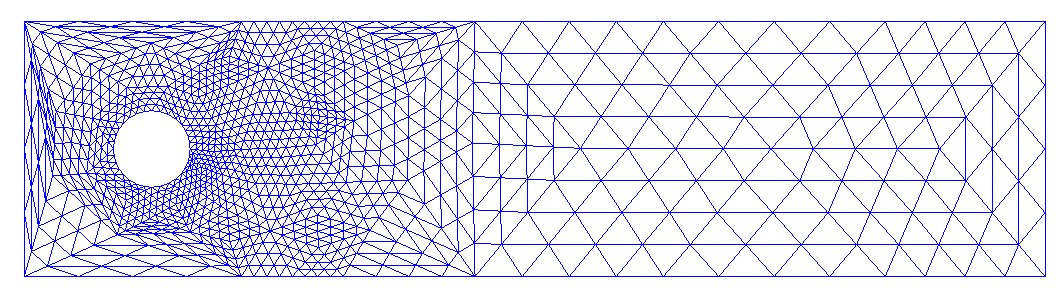
\includegraphics[scale=0.3]{figures/dolfin_plot_0.png} 

\vspace{-3mm}\hspace{60mm}Figure 1.\\\\
The most relevant feature of the flow, at moderate values of the Reynolds number is the 
onset of a time-periodic regime characterized by alternate vortex shedding, known as 
the von K\'arm\'an vortex street.

In low turbulence, tall buildings can produce a K\'arm\'an street so long as the structure 
is uniform along its height. In urban areas where there are many other tall nearby 
structures the turbulence produced by these prevents the formation of coherent vortices.
Periodic crosswind forces set up by vortices along object's sides can be highly undesirable, 
and hence it is important for engineers to account for the possible effects of vortex 
shedding when designing a wide range of structure.
\footnote{http://en.wikipedia.org/wiki/K\'arm\'an\_vortex\_street}

\hspace{35mm}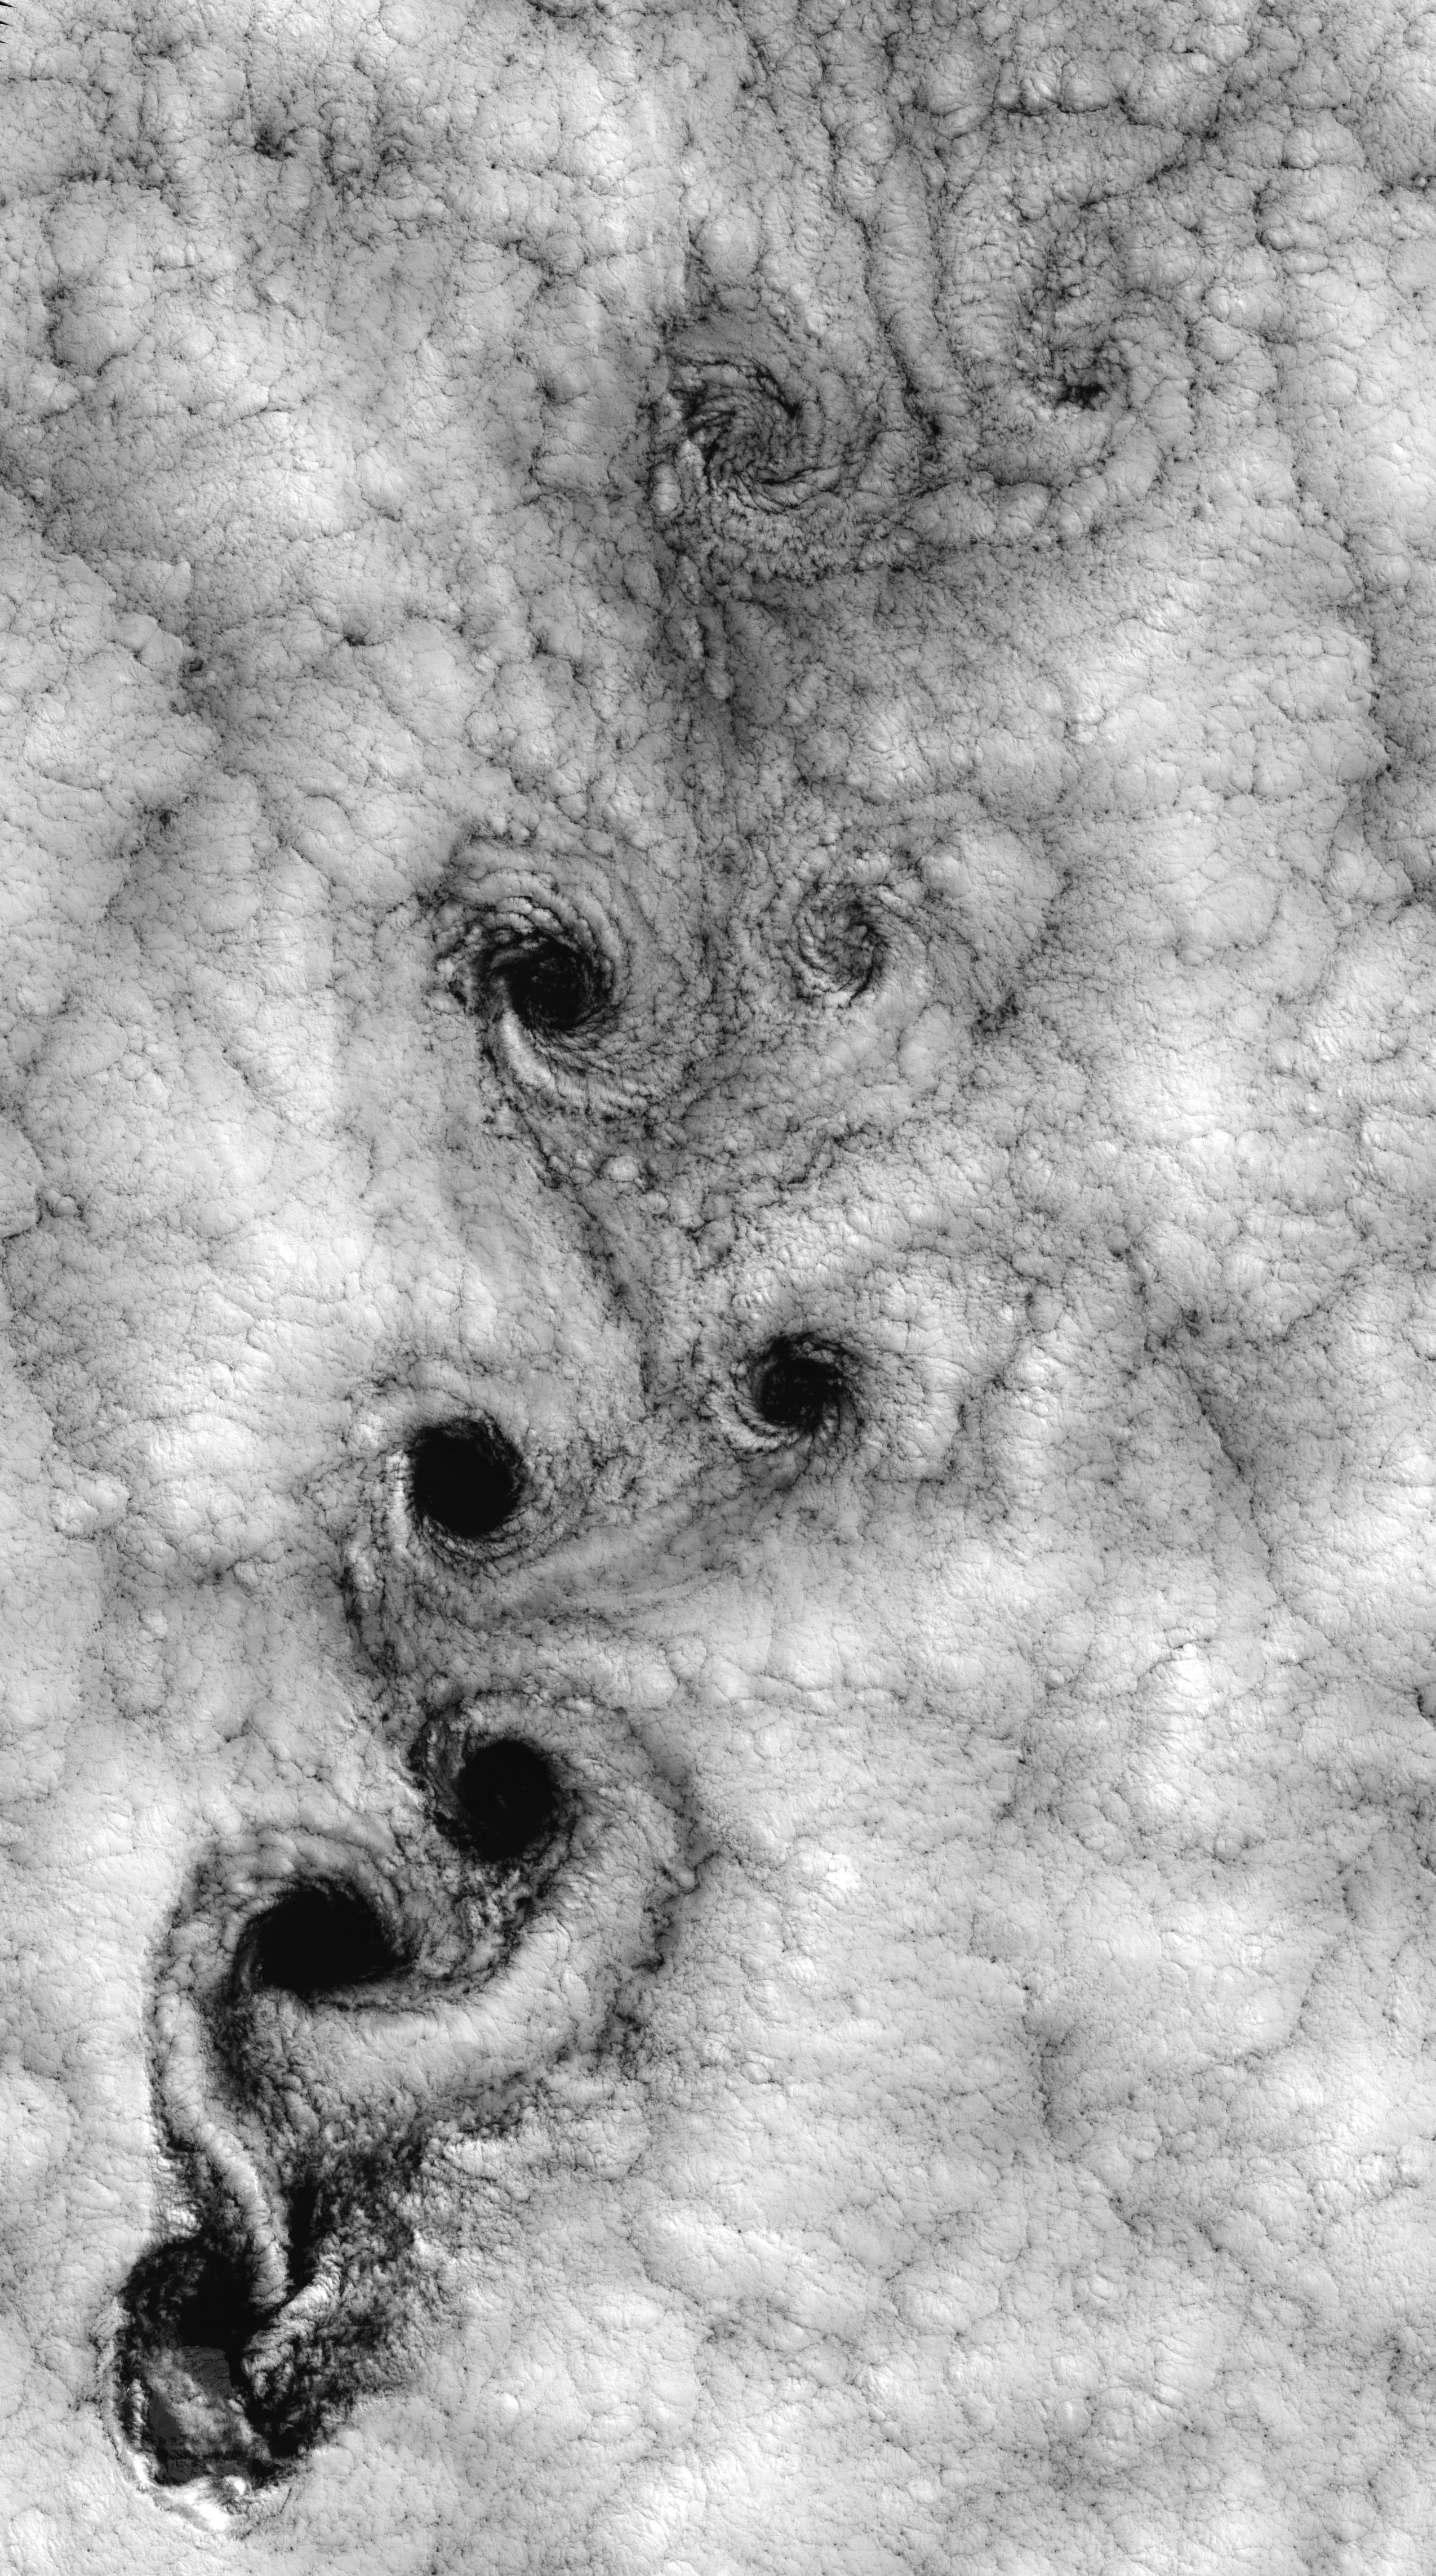
\includegraphics[scale=0.06]{figures/vonKarmanStreetinNature.jpg}

Figure 2 : \tiny{K\'arm\'an vortex street caused by wind flowing around the Juan 
Fern\'andez Islands off the Chilean coast.} \footnote{Taken from the wikipedia article.}
\normalsize{}


%%%%%%%%%%%%%%%% Channel with high resolution at boundaris %%%%%%%%%%%%%%%%%%
\subsection{Channel with high resolution at moving boundary} 
In fluid dynamics, Couette flow is the laminar flow of a viscous fluid in the space between 
two parallel plates, one of which is moving relative to the other. The mesh has been made
to take into account the movement of the top plate, while the bottom plate remains fixed.
For such flows the steady solution is given as 

\hspace{25mm}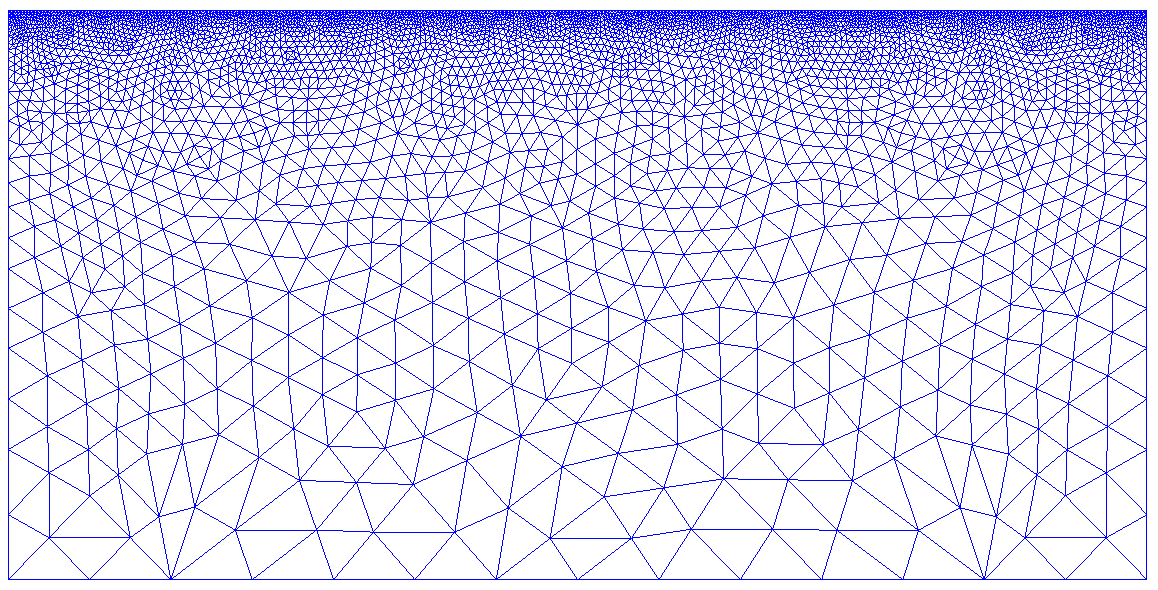
\includegraphics[scale=0.2]{figures/dolfin_plot_1.png} 

\vspace{-1mm}\hspace{60mm}Figure 3.\\

\begin{align}
\label{steadyCouette}
u(y) = \frac{U}{2} \left(1 + \frac{y}{h} \right)
\end{align}
where the length of the width is 2h and the velocity of the top boundary is given as a 
constant U. For such flows, a coarse mesh is sufficient. However, we intend to simulate
the unsteady problem, i.e the top boundary velocity starts at zero is suddenly
increased to U. There exist an analytical solution for such a flow as well. This comes
in handy when we want to see how well our solver approximates the solution by 
looking at the error between the exact solution and the discrete solution. The 
unsteady Couette flow solution is \cite{12}
\begin{align}
\label{unsteadyCouette}
u(y,t) = U\left(1 - \operatorname{erf}\left(\frac{1}{2\sqrt{\nu t}}\right) \right),
\end{align}
where $\operatorname{erf}$ is the error function, defined as
\begin{align*}
\operatorname{erf}(x) = \frac{2}{\sqrt{\pi}}\int_{0}^x e^{-t^2}\,\mathrm dt.
\end{align*}


%%%%%%%%%%%%%%%%%%%% Backward Facing step %%%%%%%%%%%%%%%%%%%%%%%%
\subsection{Backward facing step}
Separation and reattachment of turbulent flows occur in many practical engineering 
applications. In these situations, the flow experiences an adverse pressure gradient, 
i.e. the pressure increases in the direction of the flow, which causes the boundary 
layer to separate from the solid surface. The flow subsequently reattaches downstream 
forming a recirculation bubble. Among the flow geometries used for the studies of 
separated flows, the most frequently selected is the backward-facing step.\cite{13}\\

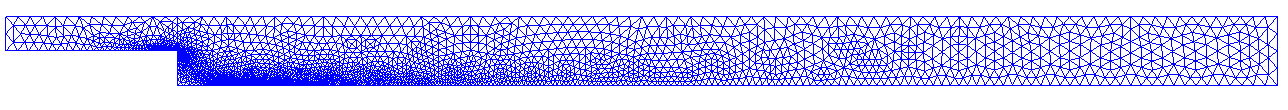
\includegraphics[scale=0.3]{figures/dolfin_plot_2.png}

\vspace{-3mm}\hspace{60mm}Figure 4.\\\\

\hspace{15mm}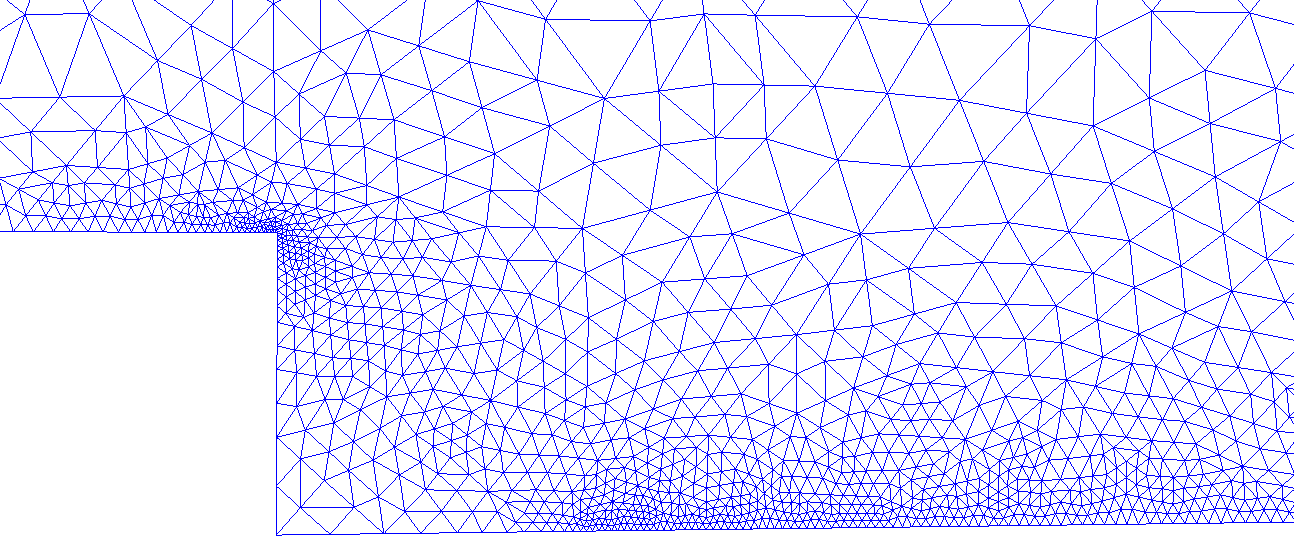
\includegraphics[scale=0.20]{figures/dolfin_plot_3.png}

\vspace{-1mm}\hspace{50mm}Figure 5 : \scriptsize{A close up of the corner.}\\\\



%%%%%%%%%%%%%%%%%%%%%%%%%%%%%%%%%%%%%%%%%%%%%%%%%%%%%
%%%%%%%%%%%%%%%%%%%    Appendices   %%%%%%%%%%%%%%%%%%%%%%
%%%%%%%%%%%%%%%%%%%%%%%%%%%%%%%%%%%%%%%%%%%%%%%%%%%%%
\newpage
\appendix

%%%%%%%%%%%%%%%%%%%%%%%%%%%%%%%%%%%%%%%%%%%%%%%%%%%%%%%%%%
%%%%%%%%%%%%%%% Derivations of NS weak form %%%%%%%%%%%%%%%%%%%%%
%%%%%%%%%%%%%%%%%%%%%%%%%%%%%%%%%%%%%%%%%%%%%%%%%%%%%%%%%%
\section{Derivation of the Navier-Stokes Weak Formulation}
In this section, we will derive the weak formulation listed as equations \eqref{weakNS} - 
\eqref{weakContinuity}.
For the sake of the clarity, we list the incompressible Navier-Stokes equations 
\begin{align}
\label{NSagain}
\frac{\partial\mathbf{u}}{\partial t} + \mathbf{u}\cdot\nabla \mathbf{u} &= 
-\frac{1}{\rho}  \nabla p  + 
\nabla \cdot \left[\nu \left(\nabla\mathbf{u} + \nabla\mathbf{u}^T \right)  \right]
+ \mathbf{f}, \\
\label{Continuityagain}
\nabla \cdot\mathbf{u} &= 0.
\end{align}
The unsteady incompressible Navier-Stokes equations \eqref{NSagain}-\eqref{Continuityagain} 
are defined on the time interval [0,T], and the domain $\Omega\subset\mathbb{R}^d $
(d = 2,3) bounded by a sufficiently regular boundary $\partial  \Omega = \Gamma_D \cup 
\hspace{1mm}\Gamma_N$, where $\Gamma$ consists of the Dirichlet and Neumann boundary.
The trial funcitons are $(\mathbf{u},p) \in\text{VxQ}$, where V $= [\text{H}^1(\Omega)]^d$ and 
Q$=\text{L}^2$. Define test functions \textbf{v},q $\in$ VxQ, and multiply \eqref{NSagain} with 
\textbf{v}, and \eqref{Continuityagain} with q, and integrate over the domain $\Omega$
\begin{align}
\label{derivationNS1}
\int_\Omega\frac{\partial\mathbf{u}}{\partial t} \cdot \mathbf{v}\,\mathrm d\mathbf{x} +
\int_\Omega (\mathbf{u}\cdot\nabla \mathbf{u}) \cdot \mathbf{v}\,\mathrm d\mathbf{x} &= 
-\int_\Omega \frac{1}{\rho}  \nabla p \cdot \mathbf{v}\,\mathrm d\mathbf{x}
+ \int_\Omega \nabla \cdot \left[\nu \left(\nabla\mathbf{u} + \nabla\mathbf{u}^T \right)  
\right] \cdot \mathbf{v}\,\mathrm d\mathbf{x}
+ \int_\Omega \mathbf{f} \cdot \mathbf{v}\,\mathrm d\mathbf{x},\\
\label{derivationContinuity1}
\int_\Omega (\nabla \cdot \mathbf{u}) q \hspace{1mm}\,\mathrm d\mathbf{x} &= 0.
\end{align}
Next we perform integration by parts on the diffusion and the pressure gradient term :
\begin{align}
\label{pressureIBP}
-\int_\Omega \frac{1}{\rho}  \nabla p \cdot \mathbf{v} d\mathbf{x} &=
\frac{1}{\rho}\int_\Omega p\nabla \cdot \mathbf{v} d\mathbf{x} 
- \frac{1}{\rho} \int_{\partial\Omega} p \mathbf{v \cdot n} ds \\
\label{diffusionIBP}
\int_\Omega \nabla \cdot \left[\nu \left(\nabla\mathbf{u} + \nabla\mathbf{u}^T \right)  
\right] \cdot \mathbf{v} d\mathbf{x} &=
-\int_\Omega \left[\nu \left(\nabla\mathbf{u} + \nabla\mathbf{u}^T \right)  
\right] : \nabla\mathbf{v} d\mathbf{x} 
+ \nu \int_{\partial \Omega} \left(\nabla\mathbf{u} + \nabla\mathbf{u}^T \right) \cdot 
\mathbf{v} \cdot \mathbf{n} ds 
\end{align}
where ds is a surface measure and \textbf{n} the normal vector; normal to the surface 
$\partial \Omega$. Inserting \eqref{pressureIBP}-\eqref{diffusionIBP} in \eqref{derivationNS1} :
\begin{align}
\label{derivationNS2}
\int_\Omega\frac{\partial\mathbf{u}}{\partial t} \cdot \mathbf{v}\,\mathrm d\mathbf{x}
+ \int_\Omega (\mathbf{u}\cdot\nabla \mathbf{u}) \cdot \mathbf{v}\,\mathrm d\mathbf{x}
- \frac{1}{\rho}\int_\Omega  p\nabla \cdot \mathbf{v}\,\mathrm d\mathbf{x} 
+ \int_\Omega \left[\nu \left(\nabla\mathbf{u} + \nabla\mathbf{u}^T \right)  
\right] : \nabla \mathbf{v}\,\mathrm d\mathbf{x}
&=  \\ \notag
- \frac{1}{\rho} \int_{\partial\Omega} p \mathbf{v \cdot n}\,\mathrm ds
+ \nu \int_{\partial \Omega} \left(\nabla\mathbf{u} + \nabla\mathbf{u}^T \right) \cdot 
\mathbf{v} \cdot \mathbf{n}\,\mathrm ds 
+ \int_\Omega \mathbf{f} \cdot \mathbf{v}\,\mathrm d\mathbf{x}.
\end{align}
Collecting the boundary terms from \eqref{derivationNS2} :
\begin{align}
\label{weakBoundary}
\int_{\partial\Omega}
\mathbf{v} \cdot \underbrace{\left[
\nu \left(\nabla\mathbf{u} + \nabla\mathbf{u}^T \right) 
- \frac{1}{\rho} p I \right]}_{= \sigma (\text{see eq.} \eqref{cauchyStress})}
 \cdot\mathbf{n}\,\mathrm ds 
&= \int_{\partial\Omega} \mathbf{\sigma \cdot v \cdot n}\,\mathrm ds.
\end{align}
Setting this to zero on the inflow/outflow boundaries ($\partial \Omega\backslash\Gamma_N$) is 
called pseudo-traction or a do-nothing boundary condition. It is often used on outlets where we 
are simply interested in letting the fluid escape with as little interference of boundary conditions 
as possible. It is called do-noting because you don’t have to do anything to enforce it.
\footnote{ http://www.uio.no/studier/emner/matnat/math/MEK4300/v13/undervisningsmateriale/lecturenotes.pdf}

We finally end up with the problem, find $(\mathbf{u},p) \in\text{VxQ}$ such that
\begin{align*}
\int_\Omega\frac{\partial\mathbf{u}}{\partial t} \cdot \mathbf{v}\,\mathrm d\mathbf{x}
+ \int_\Omega \left[\nu \left(\nabla\mathbf{u} + \nabla\mathbf{u}^T \right)  
\right] : \nabla \mathbf{v}\,\mathrm d\mathbf{x}
&= \frac{1}{\rho}\int_\Omega  p\nabla \cdot \mathbf{v}\,\mathrm d\mathbf{x} 
- \int_\Omega (\mathbf{u}\cdot\nabla \mathbf{u}) \cdot \mathbf{v}\,\mathrm d\mathbf{x}
+ \int_\Omega \mathbf{f} \cdot \mathbf{v}\,\mathrm d\mathbf{x}, \\
\int_\Omega (\nabla \cdot \mathbf{u}) q \hspace{1mm}\,\mathrm d\mathbf{x} &= 0,
\end{align*}
which is the result we have listed as equation \eqref{weakNS} and \eqref{weakContinuity}.



%%%%%%%%%%%%%%%%%%%%%%%%%%%%%%%%%%%%%%%%%%%%%%%%%%%%%%%%%%
%%%%%%%%%%% Derivations leading to the k-epsilon model %%%%%%%%%%%%%%%
%%%%%%%%%%%%%%%%%%%%%%%%%%%%%%%%%%%%%%%%%%%%%%%%%%%%%%%%%%
\section{Derivations leading to the k-$\varepsilon$ model}

For convenience, we will first start by defining some well-worn symbols and 
notations that are familiar for the purpose of the subject. 

The symbol $\tilde{u}_{i}$ will be used for the instantaneous velocity vector :
\begin{equation}
\label{1}
\tilde{u}_{i}=\left[\begin{array}{c}
\tilde{u}(\boldsymbol{x},t)\\
\tilde{v}(\boldsymbol{x},t)\\
\tilde{w}(\boldsymbol{x},t)
\end{array}\right]
\end{equation}
where $\boldsymbol{x}=\boldsymbol{x}(x,y,z)$ in cartecian coordinates
or $\boldsymbol{x}=\boldsymbol{x}(r,\theta,z)$ in polar coordinates
depending on the practical purpose. Further we will use $u_{i}$ for
fluctuating velocities, and $U_{i}$ for the mean velocities. Same
reasoning for the instantaneous, fluctuating and the mean pressure,
respectively $\tilde{p}_{i}$, $p_{i}$ and $P_{i}$. The instantaneous
velocities can be decomposed as following:

\begin{equation}
\label{2}
\tilde{u}_{i}(\boldsymbol{x},t)=U_{i}(\boldsymbol{x},t)+u_{i}(\boldsymbol{x},t)
\end{equation}
Where $U_{i}\equiv\overline{\tilde{u}}$, i.e averaged mean instantaneous
velocity. Similarly with the instantaneous pressure where $P_{i}\equiv\overline{\tilde{p}}_{i}$
is the averaged mean instantaneous pressure. 


%%%%%%%%%%%%%%%%%% Derivations of RANS %%%%%%%%%%%%%%%%%%%%%
\subsection{Derivations of the Reynolds Averaged Navier Stokes equations}

Starting from the instantaneous momentum equation i.e. The Navier-Stokes
equation, and the continuity equations for an incompressible fluid:

\begin{equation}
\label{3}
\frac{\partial\widetilde{u}_{i}}{\partial t}+\tilde{u}_{j}\frac{\partial\widetilde{u}_{i}}{\partial x_{j}}
=-\frac{1}{\rho}\tilde{p}+\nu\frac{\partial^{2}\tilde{u}_{i}}{\partial x_{j}\partial x_{j}}
\end{equation}


\begin{equation}
\label{4}
\frac{\partial u_{i}}{\partial x_{i}}=0
\end{equation}

First we will assure that the continuity equation is fulfilled. By
inserting the decomposed intantaneous velocities eq \eqref{2} in the continuity
equation \eqref{4}, and then taking the average, we get 
\begin{eqnarray}
\label{5}
\overline{\frac{\partial(U_{i}+u_{i})}{\partial x_{i}}} & = & \frac{\partial\overline{(U_{i}+u_{i})}}{\partial x_{i}}\nonumber \\
 & = & \frac{\partial(\overline{U}_{i}+\overline{u}_{i})}{\partial x_{i}}\nonumber \\
 & = & \frac{\partial(U_{i}+0)}{\partial x_{i}}\nonumber \\
\frac{\partial(U_{i})}{\partial x_{i}} & = & 0
\end{eqnarray}
Which mean that the continuity equation is satisfied. No let us insert
equation \eqref{2} in the Navier-Stokes equation \eqref{3}, and then taking the
average. 
\begin{equation}
\label{6}
\frac{\partial(U_{i}+u_{i})}{\partial t}+(U_{j}+u_{j})\frac{\partial(U_{i}+u_{i})}{\partial x_{j}}
=-\frac{1}{\rho}\frac{\partial(P+p)}{\partial x_{i}}+\nu\frac{\partial^{2}(U_{i}+u_{i})}{\partial x_{j}\partial x_{j}}
\end{equation}

\[
\overline{\frac{\partial(U_{i}+u_{i})}{\partial t}+(U_{j}+u_{j})\frac{\partial(U_{i}+u_{i})}{\partial x_{j}}
=-\frac{1}{\rho}\frac{\partial(P+p)}{\partial x_{i}}+\nu\frac{\partial^{2}(U_{i}+u_{i})}{\partial x_{j}\partial x_{j}}}
\]


\[
\overline{\frac{\partial(U_{i}+u_{i})}{\partial t}+(U_{j}+u_{j})\frac{\partial(U_{i}+u_{i})}{\partial x_{j}}}
=\overline{-\frac{1}{\rho}\frac{\partial(P+p)}{\partial x_{i}}+\nu\frac{\partial^{2}(U_{i}+u_{i})}{\partial x_{j}\partial x_{j}}}
\]

\[
\overline{\frac{\partial(U_{i}+u_{i})}{\partial t}}+\overline{(U_{j}+u_{j})\frac{\partial(U_{i}+u_{i})}{\partial x_{j}}}
=-\frac{1}{\rho}\overline{\frac{\partial(P+p)}{\partial x_{i}}}+\nu\overline{\frac{\partial^{2}(U_{i}+u_{i})}{\partial x_{j}\partial x_{j}}}
\]
\begin{equation}
\label{7}
\frac{\partial}{\partial t}(\overline{U_{i}}=U_{i}+\overline{u_{i}}=0)+\overline{(U_{j}+u_{j})\frac{\partial(U_{i}+u_{i})}{\partial x_{j}}
}=-\frac{1}{\rho}\frac{\partial}{\partial x_{i}}(\overline{P}=P+\overline{p}=0)+\nu\frac{\partial^{2}(\overline{U_{i}}+\overline{u_{i}})}{\partial x_{j}\partial x_{j}}
\end{equation}
Before handling the average of the convective term, let us employ
the continuity equation to simplify this expression:
\begin{equation}
\label{8}
(U_{j}+u_{j})\frac{\partial(U_{i}+u_{i})}{\partial x_{j}}=\frac{\partial(U_{i}+u_{i})(U_{j}+u_{j})}{\partial x_{j}}
\end{equation}
Using the rule: $\overline{U_{i}u_{i}}=\overline{U_{i}}\overline{u_{i}}=0$.
Averaging \eqref{7}
\begin{eqnarray*}
\frac{\partial}{\partial x_{j}}\overline{(U_{i}+u_{i})(U_{j}+u_{j})} & = & \frac{\partial}{\partial x_{j}}(U_{i}U_{j}+u_{i}u_{j})\\
 & = & \frac{\partial}{\partial x_{j}}(U_{i}U_{j})+\frac{\partial}{\partial x_{j}}(\overline{u_{i}u_{J}})
\end{eqnarray*}
Now we can finally insert this expression into equation \eqref{6}, and after
rearraging some terms we obtain the Reynolds average Navier-Stokes
equation.

\begin{equation}
\label{9}
\frac{\partial U_{i}}{\partial t}+U_{j}\frac{\partial U_{i}}{\partial x_{j}}
=-\frac{1}{\rho}\frac{\partial P}{\partial x_{i}}+\nu\frac{\partial^{2}U_{i}}{\partial x_{j}\partial x_{j}}-\frac{\partial}{\partial x_{j}}(\overline{u_{i}u_{J}})
\end{equation}
The last term on the right hand side of the equation is the Reynolds
$\frac{\partial}{\partial x_{j}}(\overline{u_{i}u_{J}})$ is the Reynolds
stress tensor that needs some more cumbersome processing which we
will come back to, but first we will derive the fluctuating momentum
equation. 


%%%%%%%%% Fluctuating Momentum equation %%%%%%%%%%%
\subsection{The Fluctuating Momentum Equation}

By substracting RANS equations \eqref{9} from the averaged Navier-Stokes equation
\eqref{6}, and rearranging some terms, we can show that the flutuating momentum
equation becomes: 
\begin{equation}
\label{10}
\frac{\partial u_{i}}{\partial t}+U_{j}\frac{\partial u_{i}}{\partial x_{j}}+u_{j}\frac{\partial U_{i}}{\partial x_{j}}+\frac{\partial}{\partial x_{j}}(u_{i}u_{j}-(\overline{u_{i}u_{J}})
=-\frac{1}{\rho}\frac{\partial p}{\partial x_{i}}+\nu\frac{\partial^{2}u_{i}}{\partial x_{j}\partial x_{j}}
\end{equation}
In order to show that the fluctuating velocity field is divergence free,
we can employ the definition of continuity equation for the instantaneous
velocity field, \eqref{2}, and the averaged velocity field, \eqref{4}. Subtracting
\eqref{2} from \eqref{4}
\begin{equation}
\label{11}
\frac{\partial u_{i}}{\partial x_{i}}=\frac{\partial\tilde{u}_{i}}{\partial x_{i}}-\frac{\partial U_{i}}{\partial x_{i}}=0
\end{equation}
Notice that since the partial derivative is a linear operator, we can rearrange 
the terms instead by using the definition \eqref{6} instead.


%%%%%%%%%% Derivations of stress transport equations %%%%%%%%%%%%%%%%%%
\subsection{The derivations of the Reynolds Stress Transport Equations}

In order to derive the Reynolds stress transport equation, we need
to perform the following steps :
\begin{enumerate}
\item Multiply equation \eqref{10} with $u_k$ and take the average of the resulting
equation \eqref{11}.
\item Interchange the indices i and k, and add the resulting interchanged
equation \eqref{12} to the averaged equation from step 1.
\end{enumerate}

\vspace{5mm}\hspace{-5mm}\textbf{Step 1} \\
Mutiplying equation \eqref{10} with $u_{k}$:
\[
u_{k}\left[\frac{\partial u_{i}}{\partial t}+U_{j}\frac{\partial u_{i}}{\partial x_{j}}+u_{j}\frac{\partial U_{i}}{\partial x_{j}}+\frac{\partial}{\partial x_{j}}(u_{i}u_{j}-(\overline{u_{i}u_{j}})\right]
=-\frac{1}{\rho}\frac{\partial p}{\partial x_{i}}+\nu\frac{\partial^{2}u_{i}}{\partial x_{j}\partial x_{j}}
\]
Take the average:

\[
\overline{u_{k}\frac{\partial u_{i}}{\partial t}}+\overline{u_{k}U_{j}\frac{\partial u_{i}}{\partial x_{j}}}+\overline{u_{k}u_{j}\frac{\partial U_{i}}{\partial x_{j}}}+\overline{u_{k}\frac{\partial}{\partial x_{j}}(u_{i}u_{j}-(\overline{u_{i}u_{j}})}=-\frac{1}{\rho}\overline{u_{k}\frac{\partial p}{\partial x_{i}}}+\nu\overline{u_{k}\frac{\partial^{2}u_{i}}{\partial x_{j}\partial x_{j}}}
\]
We will show that this term $(\overline{u_{i}u_{j}})$ on the left
hand side will fall out, because $\overline{u_{k}}=0$, then 
\[
\overline{u_{k}\overline{u_{i}u_{j}}}=\overline{u_{k}}\overline{\overline{u_{i}u_{j}}}=0
\]
Further, the $U_{j}$ is interchangable so that it can be extracted
out, and we get
\begin{equation}
\label{12}
\overline{u_{k}\frac{\partial u_{i}}{\partial t}}+U_{j}\overline{\frac{\partial}{\partial x_{j}}(u_{i}u_{k})}=-\frac{1}{\rho}\overline{u_{k}\frac{\partial p}{\partial x_{i}}}+\nu\overline{u_{k}\frac{\partial^{2}u_{i}}{\partial x_{j}\partial x_{j}}}-\overline{u_{k}u_{j}}\frac{\partial U_{i}}{\partial x_{j}}-\overline{u_{k}u_{j}\frac{\partial u_{i}}{\partial x_{j}}}
\end{equation}
The last term on right hand side follows by the continuity equation.
\\\\
\textbf{Step 2} \\
For equation \eqref{12} interchange indices i and k (as they are both free
indices) :
\begin{equation}
\label{13}
\overline{u_{i}\frac{\partial u_{k}}{\partial t}}+U_{j}\overline{\frac{\partial}{\partial x_{j}}(u_{k}u_{i})}=-\frac{1}{\rho}\overline{u_{i}\frac{\partial p}{\partial x_{k}}}+\nu\overline{u_{i}\frac{\partial^{2}u_{k}}{\partial x_{j}\partial x_{j}}}-\overline{u_{i}u_{j}}\frac{\partial U_{k}}{\partial x_{j}}-\overline{u_{i}u_{j}\frac{\partial u_{k}}{\partial x_{j}}}
\end{equation}
Adding\eqref{12} to \eqref{11}, and noticing that $\frac{\partial(u_{i}u_{k})}{\partial t}=u_{k}\frac{\partial u_{i}}{\partial t}+u_{i}\frac{\partial u_{k}}{\partial t}$:
\begin{eqnarray}
\label{14}
\frac{\partial}{\partial t}\overline{(u_{i}u_{k})}+U_{j}\overline{\frac{\partial}{\partial x_{j}}(u_{i}u_{k})} & = & -\frac{1}{\rho}\left(\overline{u_{i}\frac{\partial p}{\partial x_{k}}}+\overline{u_{k}\frac{\partial p}{\partial x_{i}}}\right)+\nu\left(\overline{u_{i}\frac{\partial^{2}u_{k}}{\partial x_{j}\partial x_{j}}}+\overline{u_{k}\frac{\partial^{2}u_{i}}{\partial x_{k}\partial x_{k}}}\right)\nonumber \\
 &  & -\overline{u_{i}u_{j}}\frac{\partial U_{k}}{\partial x_{j}}-\overline{u_{k}u_{j}}\frac{\partial U_{i}}{\partial x_{j}}-\overline{u_{i}u_{j}\frac{\partial u_{k}}{\partial x_{j}}}-\overline{u_{k}u_{j}\frac{\partial u_{i}}{\partial x_{j}}}
\end{eqnarray}
We can further simplify this expression. Let us rst start with the
term with kinematic viscosity(the Laplacian terms). In order to simplify
this expression, we need to use the product rule, and perform some
manipulations with the new expressions :
\begin{eqnarray}
\frac{\partial}{\partial x_{j}}\left(u_{i}\frac{\partial}{\partial x_{j}}(u_{k})\right) & = & \underbrace{\frac{\partial(u_{i})}{\partial x_{j}}\frac{\partial(u_{k})}{\partial x_{j}}}+u_{i}\frac{\partial^{2}u_{k}}{\partial x_{j}\partial x_{j}}\nonumber \\ 
 & \Downarrow & \frac{\partial(u_{k})}{\partial x_{j}}\frac{\partial(u_{i})}{\partial x_{j}}\nonumber \\ \label{15}
u_{i}\frac{\partial^{2}u_{k}}{\partial x_{j}\partial x_{j}} & = & \frac{\partial}{\partial x_{j}}\left(u_{i}\frac{\partial}{\partial x_{j}}(u_{k})\right)-\frac{\partial(u_{i})}{\partial x_{j}}\frac{\partial(u_{k})}{\partial x_{j}}\\
\frac{\partial^{2}}{\partial x_{j}\partial x_{j}}(u_{i}u_{k}) & = & \frac{\partial}{\partial x_{j}}\left(u_{k}\frac{\partial}{\partial x_{j}}(u_{i})\right)+\frac{\partial}{\partial x_{j}}\left(u_{i}\frac{\partial}{\partial x_{j}}(u_{k})\right)\nonumber \\
 & \Downarrow\nonumber \\ \label{16}
\frac{\partial}{\partial x_{j}}\left(u_{i}\frac{\partial}{\partial x_{j}}(u_{k})\right) & = & \frac{\partial^{2}}{\partial x_{j}\partial x_{j}}(u_{i}u_{k})-\frac{\partial}{\partial x_{j}}\left(u_{k}\frac{\partial}{\partial x_{j}}(u_{i})\right)
\end{eqnarray}
Insert \eqref{16} into \eqref{15} : 
\begin{eqnarray}
u_{i}\frac{\partial^{2}u_{k}}{\partial x_{j}\partial x_{j}} & = & \frac{\partial^{2}}{\partial x_{j}\partial x_{j}}(u_{i}u_{k})-\frac{\partial}{\partial x_{j}}\left(u_{k}\frac{\partial}{\partial x_{j}}(u_{i})\right)-\frac{\partial}{\partial x_{j}}\left(u_{i}\frac{\partial}{\partial x_{j}}(u_{k})\right)\nonumber \\ \label{17}
 & = & \frac{\partial}{\partial x_{j}}\left(\frac{\partial}{\partial x_{j}}(u_{i}u_{k})-u_{k}\frac{\partial}{\partial x_{j}}(u_{i})\right)-\frac{\partial}{\partial x_{j}}u_{i}\frac{\partial}{\partial x_{j}}(u_{k})
\end{eqnarray}
Performing similar calculations for $u_{k}\frac{\partial^{2}u_{i}}{\partial x_{j}\partial x_{j}}$(or
simply interchanging the i and k indices in equation \eqref{14} ) :
\begin{equation}
\label{18}
u_{k}\frac{\partial^{2}u_{i}}{\partial x_{j}\partial x_{j}}=\frac{\partial}{\partial x_{j}}\left(u_{k}\frac{\partial}{\partial x_{j}}(u_{i})\right)-\frac{\partial}{\partial x_{j}}u_{k}\frac{\partial}{\partial x_{j}}(u_{i})
\end{equation}
If we now add \eqref{16} and \eqref{17} we get 
\begin{eqnarray} \nonumber
u_{i}\frac{\partial^{2}u_{k}}{\partial x_{j}\partial x_{j}}+u_{k}\frac{\partial^{2}u_{i}}{\partial x_{j}\partial x_{j}} & = 
& \frac{\partial}{\partial x_{j}}\left(\frac{\partial}{\partial x_{j}}(u_{i}u_{k})
-u_{k}\frac{\partial}{\partial x_{j}}(u_{i})\right)+\frac{\partial}{\partial x_{j}}\left(u_{k}\frac{\partial}{\partial x_{j}}(u_{i})\right)
-2\frac{\partial}{\partial x_{j}}u_{i}\frac{\partial}{\partial x_{j}}(u_{k})\\ \label{19}
 & = & \frac{\partial^{2}}{\partial x_{j}\partial x_{j}}(u_{i}u_{k})
-2\frac{\partial}{\partial x_{j}}u_{i}\frac{\partial}{\partial x_{j}}(u_{k})
\end{eqnarray}
Finally due to continuity(as we have already shown that the fluctuating
velocity field is divergence free, this assumption is thus valid), the
last two terms in \eqref{14} can be simplified; again using the product rule :
\begin{equation}
\label{20}
u_{i}u_{j}\frac{\partial u_{k}}{\partial x_{j}}+u_{k}u_{j}\frac{\partial u_{i}}{\partial x_{j}}=\frac{\partial(u_{i}u_{k}u_{j})}{\partial x_{j}}
\end{equation}
Inserting equation \eqref{19} and \eqref{20} in equation \eqref{18} we get the Reynolds stress transport equation. 
\begin{eqnarray}
\label{21}
\frac{\partial}{\partial t}\overline{(u_{i}u_{k})}+U_{j}\overline{\frac{\partial}{\partial x_{j}}(u_{i}u_{k})} & = 
& -\frac{1}{\rho}\left(\overline{u_{i}\frac{\partial p}{\partial x_{k}}}+\overline{u_{k}\frac{\partial p}{\partial x_{i}}}\right)
-2\nu\overline{\left(\frac{\partial}{\partial x_{j}}u_{i}\frac{\partial}{\partial x_{j}}(u_{k})\right)}\\
 &  & -\overline{u_{i}u_{j}}\frac{\partial U_{k}}{\partial x_{j}}-\overline{u_{k}u_{j}}\frac{\partial U_{i}}{\partial x_{j}}
-\frac{\partial\overline{(u_{i}u_{k}u_{j})}}{\partial x_{j}}+\nu\frac{\partial^{2}}{\partial x_{j}\partial x_{j}}\overline{(u_{i}u_{k})}\nonumber 
\end{eqnarray}


%%%%%%%%%%%% Derivation of the k-epsilon model %%%%%%%%%%%%%%%%
\subsection{Derivation of the $k-\epsilon$ model}
In the previous subsection we derived the Reynolds stress transport equation \eqref{21} :
\begin{align*}
\partial_t (\overline{u_i u_k}) + U_j \partial_j\overline{u_i u_k} =
-\frac{1}{\rho} (\overline{u_i \partial_k p} +\overline{u_k \partial_i p} ) & 
\\ 
- 2\nu (\overline{\partial_j u_i \partial_j u_k}) & 
\\
- \overline{ u_i u_j} \partial_j U_k - \overline{ u_k u_j} \partial_j U_i
\\ 
- \partial_j\overline{ (u_i u_k u_j)} \\ 
+ \nu\partial_j \partial_j \overline{u_i u_k} .
\end{align*}
Here we have used the short notation for the partial derivatives $\partial_i$. 
Multiplying this equation by half and setting i=k, we get the following equation (after rearranging the equation) :
\begin{align*} 
\partial_t k + U_j \partial_j k &= \overbrace{\tau_{ij} \partial_j U_i}^{\text{production}}
- \overbrace{\epsilon}^{\text{dissipation}} \\
&+ \partial_j \left[ \nu \partial_j k - \underbrace{\frac{1}{2}\overline{u_i u_i u_j}}_{\hidewidth{\text{turbulent transport}}}
 -\overbrace{\frac{1}{\rho} \overline{p u_j}}^{\hidewidth{\text{pressure diffusion}}}\right]
\end{align*}
For the pressure term, we used that $\partial_j u_j= 0$. This equation is known as the 
transport equation for turbulence kinetic energy. $\epsilon$ is the dissipation per 
unit mass and is defined by the following correlation :
\begin{equation*}
\epsilon = \nu \overline{\partial_j u_i \partial_j u_i}
\end{equation*}
$\tau_{ij}$ is the Reynolds-stress tensor $-\overline{u_i u_j}$, hence the specific(or per unit mass) 
turbulence kinetic energy (or simply the turbulence kintic energy) is half the trace of the Reynolds-stress 
tensor. \\

\textbf{Reynolds-stess tensor} : RANS turbulence models must predict the Reynolds-stresses, 
which prevents closure for the averaged momentum equations. The most common way of 
predicting these stresses is to assume that the Boussinesq approximation is valid. This implies 
that the Reynolds-stess tensor is given by
\begin{equation*}
\tau_{ij} = 2\nu_T S_{ij} -\frac{2}{3} k \delta_{ij}
\end{equation*}
where $S_{ij}$ is the mean strain rate of strain tensor :
\begin{equation*}
S_{ij} = \partial_j U_i + \partial_i U_j
\end{equation*}
The RANS turbulence models of this type are referred to as eddy viscosity models. 
Assuming that Boussinesq approxmimation is valid, it follows that production P is given as
\begin{equation} \label{eq:production}
P = \left(2\nu_T S_{ij} -\frac{2}{3} k \right) \partial_j U_i
\end{equation}

\textbf{Gradient Transport Law} : The "traditional" or standard approximation made 
to represent turbulent transport of scalar quantities in a turbulent flow is given on the form 
\begin{equation*}
\frac{1}{2}\overline{u_i u_i u_j} + \frac{1}{\rho}\overline{p u_j} = -\frac{\nu_T}{\sigma_k} \partial_j k
\end{equation*}
where $\sigma_k$ is a closure coeffient and may be considered a turbulent Prandtl number.
Inserting the last two equations into the transport equation for turbulence kinetic equation 
we finally end up with equation \eqref{tbk}.

In order to derive the dissipation rate $\epsilon$ we need to perform the following calculations
\begin{enumerate}
\item Differentiate the Navier-Stokes equations by $\partial_j$, giving an equation for $\partial_j \tilde{u}_i$
\item Multiply this equation by $2\nu \partial_j u_i$
\item Take the average of the resulting equation.
\end{enumerate}
Although this procedure has been listed, we will not attempt at deriving the equation for 
dissipation rate. In \cite[page 28-29]{14}, a detailed physical interpretation is provided
for all the terms.


%%%%%%%%%%%%%%%%%%%%%%%  References %%%%%%%%%%%%%%%%%%%%%%%%%%
\newpage
\begin{thebibliography}{9}

\bibitem{1}
	David C. Wilcox, 2006.
	\emph{Turbulence Modeling for CFD, third Edition}.

\bibitem{2}
	W. P. Jones and B. E. Launder, 1972.
	\emph{The Prediction of Laminarization with a Two-Equation Model of Turbulence}.

\bibitem{3}
	Kristian Valen-Sendstad et al., MekIT'09.
	\emph{Implementing a k-$\varepsilon$ Turbulence Model in the \mbox{FEniCS} Finite Element Programming Environment}.

\bibitem{4}
	L. Quartapelle, 1993.
	\emph{Numerical Solution of the Incompressible Navier-Stokes Equations}.

\bibitem{5}
	T. J. R. Hughes et al., 1986.
	\emph{A New Finite Element Formulation for Computational Fluid Dynamics: V. Circumventing the Babu$\check{s}$ka-Brezzi Condition : 
A Stable Petrov-Galerkin Formulation of the Stokes Problem Accommodating Equal-Order Interpolations}.

\bibitem{6}
	J. L. Guermond et al., 2006.
	\emph{An overview of projection methods for incompressible flows}.

\bibitem{7}
	A. J. Chorin, 1968.
	\emph{Numerical solution of the Navier-Stokes equations}.

\bibitem{8}
	R. Temam, 1969.
	\emph{Sur l'approximation de la solution des \'equations de Navier-Stokes par la m\'ethode des pas fractionnaires}.

\bibitem{9}
	R. Rannacher, 1992.
	\emph{On chorin's projection method for the incompressible navier-stokes equations}.

\bibitem{10}
	H. P. Langtangen, et al., 2002.
	\emph{Numerical methods for incompressible viscous flow}.

\bibitem{11}
	Jie Liu, 2009.
	\emph{Open and traction boundary conditions for the incompressible Navier-Stokes equations}.

\bibitem{12}
	Frank M. White, 2006.
	\emph{Viscous Fluid Flow, third edition}.

\bibitem{13}
	P. Moin, et al., 1996.
	\emph{Direct numerical simulation of turbulent flow over a backward-facing step}.

\bibitem{14}
	Peter S. Bernard $\&$ James M. Wallace, 2002.
	\emph{Turbulent Flow : Analysis, Measurement and Prediction}.

\end{thebibliography}

\end{document}